\documentclass[12pt,twoside]{article}
\usepackage{amsmath, amssymb}
\usepackage{amsfonts}
\usepackage[active]{srcltx}
\usepackage{amssymb}
\usepackage{amscd}
\usepackage{makeidx}
\usepackage{amsthm}
\usepackage{algpseudocode}
\usepackage{algorithm}
\usepackage{xcolor}
\usepackage{listings}
\usepackage{graphicx}

\usepackage{verbatim}

%Para código en C ------------------------------------
\definecolor{gray97}{gray}{.97}
\definecolor{gray75}{gray}{.75}
\definecolor{gray45}{gray}{.45}

\lstset{ frame=Ltb,
framerule=0pt,
aboveskip=0.5cm,
framextopmargin=3pt,
framexbottommargin=3pt,
framexleftmargin=0.4cm,
framesep=0pt,
rulesep=.4pt,
backgroundcolor=\color{gray97},
rulesepcolor=\color{black},
%
stringstyle=\ttfamily,
showstringspaces = false,
basicstyle=\small\ttfamily,
commentstyle=\color{gray45},
keywordstyle=\bfseries,
%
numbers=left,
numbersep=15pt,
numberstyle=\tiny,
numberfirstline = false,
breaklines=true,
}

% minimizar fragmentado de listados
\lstnewenvironment{listing}[1][]
{\lstset{#1}\pagebreak[0]}{\pagebreak[0]}

\lstdefinestyle{consola}
{basicstyle=\scriptsize\bf\ttfamily,
backgroundcolor=\color{gray75},
}

\lstdefinestyle{C}
{language=C,
}
%------------------------------------------------------


\renewcommand{\baselinestretch}{1}
\setcounter{page}{1}
\setlength{\textheight}{21.6cm}
\setlength{\textwidth}{14cm}
\setlength{\oddsidemargin}{1cm}
\setlength{\evensidemargin}{1cm}
\pagestyle{myheadings}
\thispagestyle{empty}
\markboth{\small{Pr\'actica 1.1. Luis Enrique}}{\small{.}}
\date{}


%------------------------------------------------------
\begin{document}
\centerline{\bf Aplicaciones para comunicaciones de red, Sem: 2019-2, 3CM5, pr\'actica 1.1, Fecha: 02/02/2019}
\centerline{}
\centerline{}
\begin{center}
\Large{\textsc{Pr\'actica 1.1: SERVICIO DE TRANSFERENCIA DE ARCHIVOS}}
\end{center}
\centerline{}
\centerline{\bf {Hern\'andez Tapia Luis Enrique.}}
\centerline{}
\centerline{Escuela Superior de C\'omputo}
\centerline{Instituto Polit\'ecnico Nacional, M\'exico}
\centerline{$tapia641@gmail.com$}
\newtheorem{Theorem}{\quad Theorem}[section]
\newtheorem{Definition}[Theorem]{\quad Definition}
\newtheorem{Corollary}[Theorem]{\quad Corollary}
\newtheorem{Lemma}[Theorem]{\quad Lemma}
\newtheorem{Example}[Theorem]{\quad Example}
\bigskip

%------------------------------------------------------
\textbf{Resumen:} En esta pr\'actica se desarrolla una aplicaci\'on para seleccionar m\'ultiples archivos y enviarlos a trav\'es del protocolo TCP. \newline.
%------------------------------------------------------
\textbf{\newline Palabras clave:} TCP, IP, Sockets de flujo.
%------------------------------------------------------



%------------------------------------------------------
\section{Introducci\'on}

El env\'io de archivos a trav\'es de la red es una caracter\'istica importante para la gran mayor\'ia de las aplicaciones que hoy d\'ia se utilizan (blogs, redes sociales, mensajer\'ia instant\'anea, declaraci\'on de impuestos, educaci\'on en l\'inea, etc.), sin embargo, no todas las aplicaciones disponibles permiten el env\'io de archivos de gran tama\~no (p.e. El correo electr\'onico no permite enviar archivos de m\'as de 10 o 20 MB).
Esto hace necesario el desarrollo de aplicaciones que permitan transferir archivos sin importar el tamaño de \'estos.

\newpage
%------------------------------------------------------


\section{Desarrollo}

A partir de los programas \textbf{CArchivo} y \textbf{SArchivo} que te ser\'an proporcionados por el profesor deber\'as realizar los siguientes programas: \newline\newline 

\textbf{Instrucciones: }

\begin{itemize}
    \item El programa \textbf{Selecci\'on} implementa una caja de di\'alogo para seleccionar un archivo a trav\'es del rat\'on en el sistema de archivos local. Deber\'as modificar el c\'odigo para que te permita seleccionar m\'as de un archivo a la vez y devuelva como salida la lista con los nombres y tama\'~nos de los archivos seleccionados.
    
    \item El programa \textbf{RecibeArchivo} implementa un servidor de flujo bloqueante que realiza la recepci\'on de un archivo ya predefinido y \'este es recibido utilizando flujos orientados a byte. Deber\'as modificar el c\'odigo para que en lugar de recibir un archivo, este programa permita recibir desde uno hasta cualquier cantidad de archivos
(secuencialmente). Para esto, primero deber\'a recibir un n\'umero que indique el n\'umero de archivos que ser\'an recibidos, posteriormente, por cada archivo a ser recibido, primero se recibir\'a el nombre del archivo, luego su tama\~no en bytes y despu\'es se recibir\'a el contenido del mismo.

    \item Durante la transferencia de los archivos el usuario deber\'a visualizar el porcentaje de env\'io en pantalla. El programa \textbf{EnviaArchivo} implementa un cliente de flujo bloqueante que envía un archivo ya preestablecido y \'este es enviado usando flujos orientados a byte. Deber\'as modificar el c\'odigo para que en lugar de enviar un
solo archivo, \'este sea capaz de enviar uno o m\'as archivos que ser\'an seleccionados por el usuario a trav\'es del programa \textbf{Selecci\'on}. 

    \item Durante la transferencia de los archivos el usuario deber\'a visualizar el porcentaje de env\'io en pantalla. El programa \textbf{EnviaArchivo} implementa un cliente de flujo bloqueante que envía un archivo ya preestablecido y \'este es enviado usando flujos orientados a byte. Deber\'as modificar el c\'odigo para que en lugar de enviar un
solo archivo, \'este sea capaz de enviar uno o m\'as archivos que ser\'an seleccionados por el usuario a trav\'es del programa \textbf{Selecci\'on}. 

\newpage

Cada archivo se enviar\'a de manera individual y el proceso de envío ser\'a de la siguiente
manera: 
\newline
Primero se enviar\'a un n\'umero indicando la cantidad de archivos que ser\'an transferidos. 
\newline 
Despu\'es, de manera iterativa, por cada archivo a ser enviado se mandar\'a previamente el nombre de \'este y su tamaño en bytes.
\newline
Posteriormente el contenido del archivo.

    \item Realiza pruebas intentando enviar distintos tipos de archivo (im\'agenes, texto, ejecutables), as\'i mismo intenta enviar archivos de distintos tamaños (menos de 100KB, m\'as de 100KB y menos de 10MB, m\'as de 10MB y
menos de 200MB, m\'as de 200MB y hasta 2GB).


\end{itemize}



%------------------------------------------------------

\section{Pruebas}
Mostrando caja de di\'alogo:
\begin{figure}[h]
	\centering
	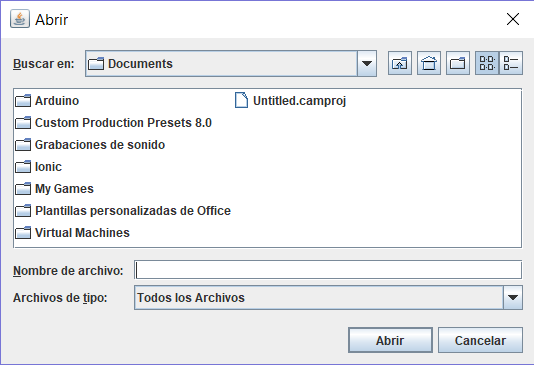
\includegraphics[width=1\textwidth]{img/JFChooser.png}
	\caption{Caja de di\'alogo para seleccionar archivos.}
\end{figure}

\newpage

Probando conexi\'on:
\begin{figure}[h]
	\centering
	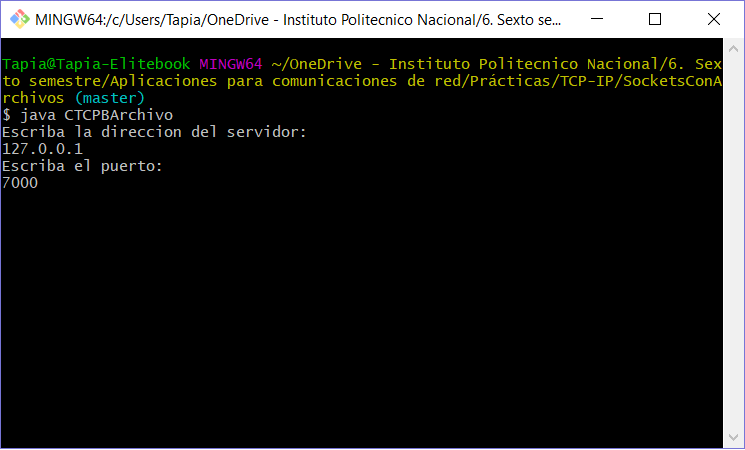
\includegraphics[width=0.8\textwidth]{img/Cliente.png}
	\caption{Cliente.}
\end{figure}

\begin{figure}[h]
	\centering
	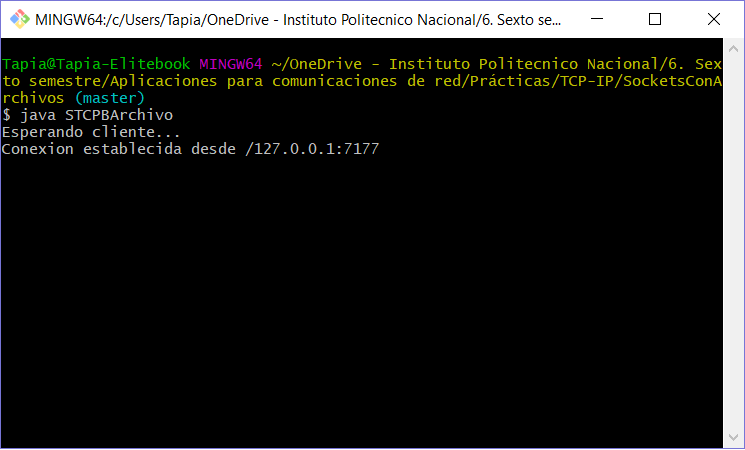
\includegraphics[width=0.8\textwidth]{img/Servidor.png}
	\caption{Servidor.}
\end{figure}

\newpage

Enviando archivos de a lo m\'as 100KB:
\begin{figure}[h]
	\centering
	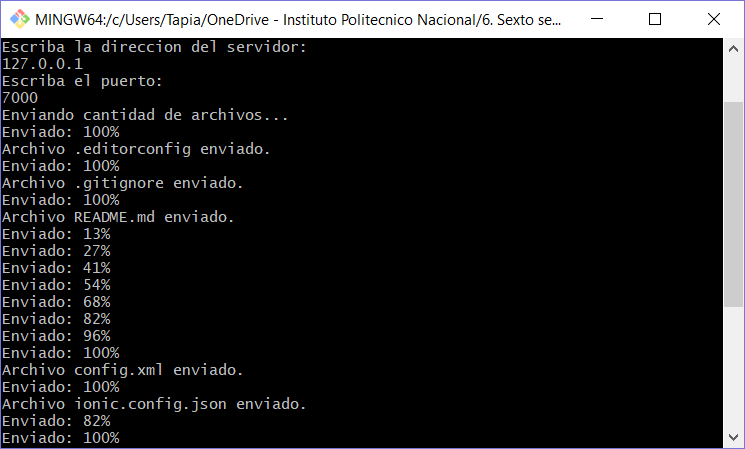
\includegraphics[width=0.8\textwidth]{img/Cliente1.png}
	\caption{Cliente.}
\end{figure}

\begin{figure}[h]
	\centering
	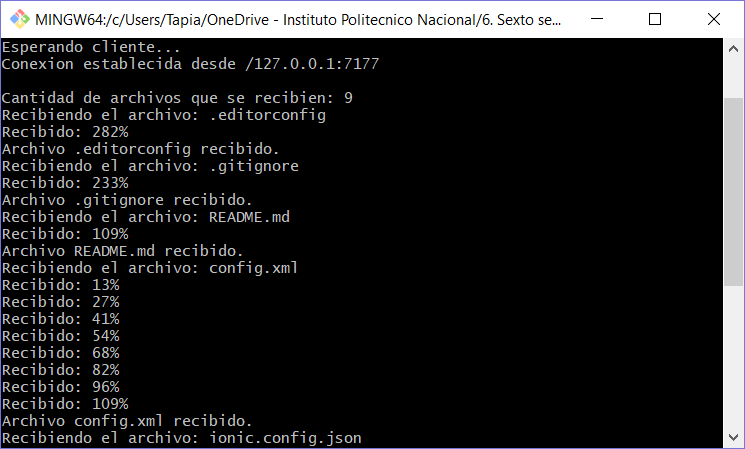
\includegraphics[width=0.8\textwidth]{img/Servidor1.png}
	\caption{Servidor.}
\end{figure}

\newpage

Enviando archivos de a lo m\'as 200MB:
\begin{figure}[h]
	\centering
	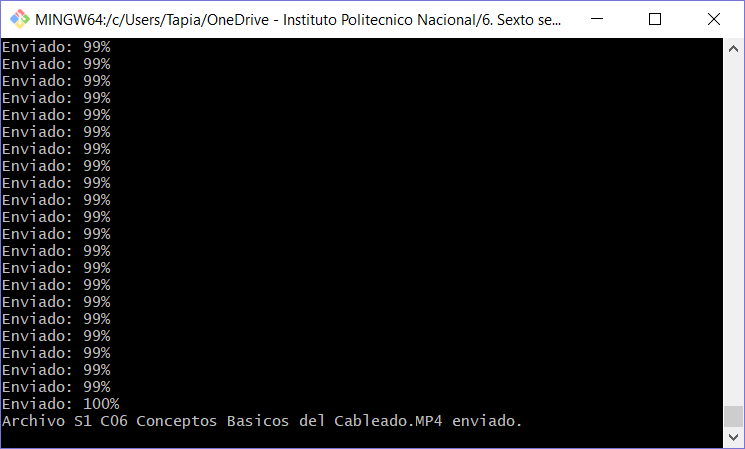
\includegraphics[width=0.8\textwidth]{img/Cliente2.png}
	\caption{Cliente.}
\end{figure}

\begin{figure}[h]
	\centering
	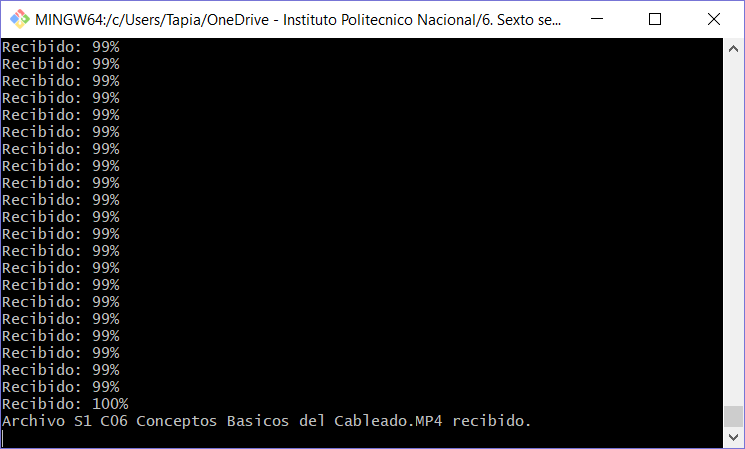
\includegraphics[width=0.8\textwidth]{img/Servidor2.png}
	\caption{Servidor.}
\end{figure}

\newpage

Enviando archivos de a lo m\'as 200MB:
\begin{figure}[h]
	\centering
	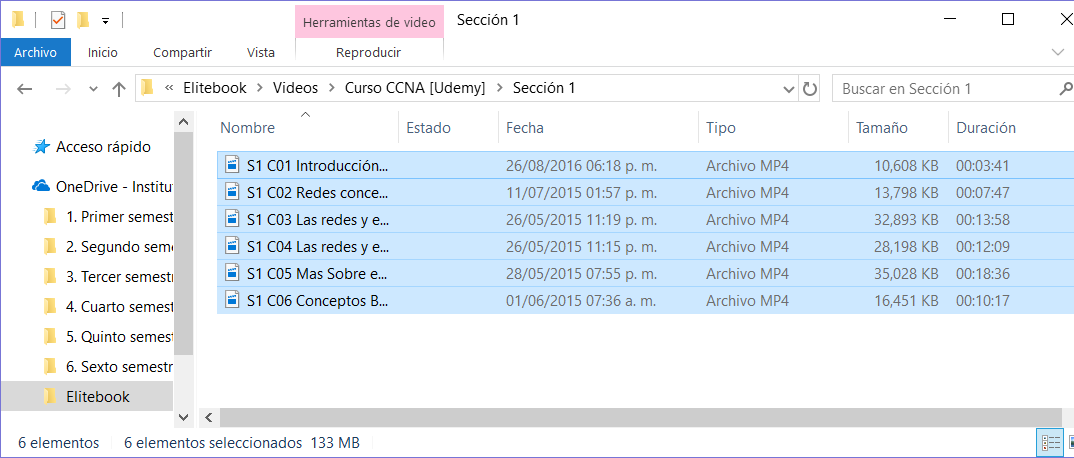
\includegraphics[width=1\textwidth]{img/ArchivosEnviados.png}
	\caption{Directorio origen.}
\end{figure}

\begin{figure}[h]
	\centering
	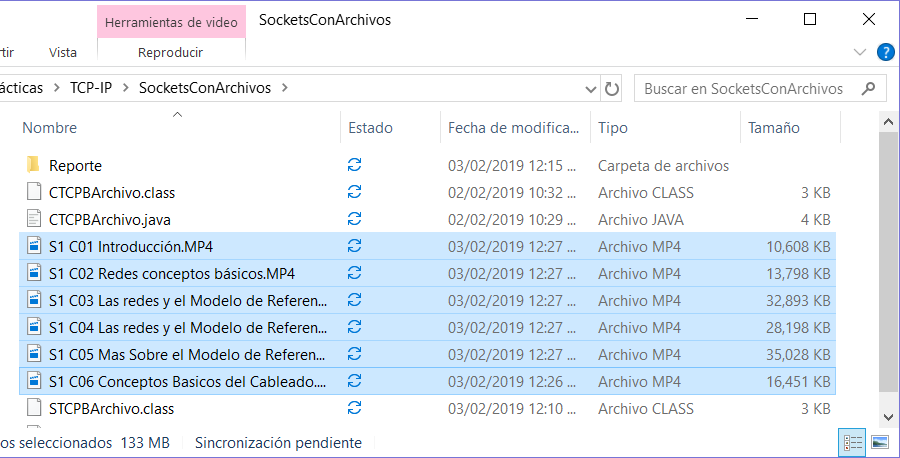
\includegraphics[width=1\textwidth]{img/ArchivosRecibidos.png}
	\caption{Directorio destino.}
\end{figure}

\newpage

Enviando archivos de m\'as 2GB:

\begin{figure}[h]
	\centering
	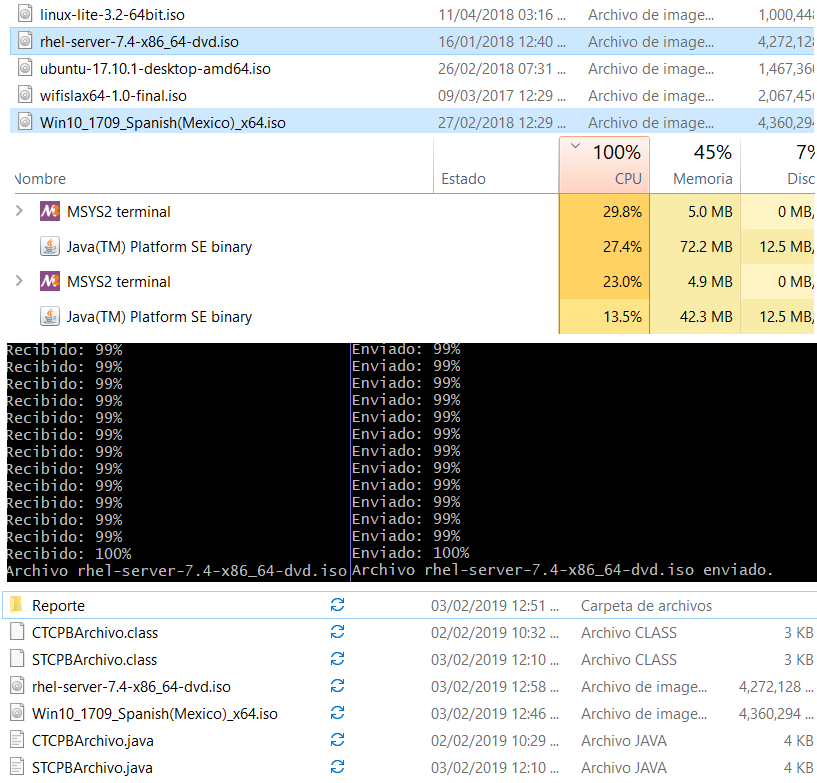
\includegraphics[width=1\textwidth]{img/CS1.png}
	\caption{Resumen de la transferencia.}
\end{figure}

\newpage
%---------------------------------------------------------------------------------
		
\section{Preguntas}

\begin{enumerate}
\item ?`Qu\'e tipo de archivos se enviaron m\'as r\'apido?
\newline \textbf{R:}

\item ?`Cu\'al fue el n\'umero m\'aximo de archivos que fue posible enviar a la vez?
\newline \textbf{R:}

\item ?`Cu\'al fue el tama\~no de archivo m\'as grande que se pudo transferir? ?`por qu\'e?
\newline \textbf{R:}

\item Si dese\'aramos enviar archivos de tama\~no muy grande, ?`qu\'e cambios ser\'ia necesario hacer con respecto a los tipos de datos usados para medir el tama\~no de los archivos, as\'i como para leer bloques de datos del archivo?
\newline \textbf{R:}


\end{enumerate}

\section{Bibliograf\'ia}
\begin{thebibliography}{X}	
\bibitem{a}  \textit{A method for the construction of minimum-redundancy codes, Proceedings of the I.R.E., sept 1952, pp 1098\-1102}

\bibitem{g} \textit{https://ronnyml.wordpress.com/2009/07/19/quicksort-en-c/}
\end{thebibliography}
\end{document}